%%%%%%%%%%%%%%%%%%%%%%% file typeinst.tex %%%%%%%%%%%%%%%%%%%%%%%%%
%
% This is the LaTeX source for the instructions to authors using
% the LaTeX document class 'llncs.cls' for contributions to
% the Lecture Notes in Computer Sciences series.
% http://www.springer.com/lncs       Springer Heidelberg 2006/05/04
%
% It may be used as a template for your own input - copy it
% to a new file with a new name and use it as the basis
% for your article.
%
% NB: the document class 'llncs' has its own and detailed documentation, see
% ftp://ftp.springer.de/data/pubftp/pub/tex/latex/llncs/latex2e/llncsdoc.pdf
%
%%%%%%%%%%%%%%%%%%%%%%%%%%%%%%%%%%%%%%%%%%%%%%%%%%%%%%%%%%%%%%%%%%%
\documentclass[runningheads]{llncs}
%\usepackage[dvips]{color}
%\usepackage{multicol}
%\usepackage{tabls}
%\usepackage{ttbox}
\usepackage{allmtt}
%\usepackage{pstricks,pst-node,pst-tree} % PS Tricks for diagrams
\setcounter{tocdepth}{3}
\usepackage{graphicx}
\usepackage{amsmath}
\usepackage{amssymb}
\usepackage{latexsym}
\usepackage{stmaryrd}
%\usepackage{mbboard}
\usepackage{xspace}
\usepackage{diagrams}
\usepackage{proof2}
\usepackage{url}


\urldef{\mailsa}\path|l.dixon@ed.ac.uk|
\urldef{\mailsb}\path|ross.duncan@comlab.ox.ac.uk|
\newcommand{\keywords}[1]{\par\addvspace\baselineskip
\noindent\keywordname\enspace\ignorespaces#1}

% -=-=-=-=-=-=-=-=-=-=-=-=-=-=-=-=-=-=-=-=-=-=-=-=-=-=-=-=-=-=-=-=-=-=-=-=-
%   Random maybe useful things...
% -=-=-=-=-=-=-=-=-=-=-=-=-=-=-=-=-=-=-=-=-=-=-=-=-=-=-=-=-=-=-=-=-=-=-=-=-
\newcommand{\cmnt}[1]{\textcolor[rgb]{ 0.8,      0,    0  }{#1}}
%\newcommand{\intabp}[2]{\parbox[t]{#1}{\raggedright{#2}\vspace{0.2cm}}}
%\newcommand{\vsmall}[1]{\footnotesize{#1}}
\newcommand{\ors}{\oplus}
\newcommand{\tensor}{\otimes}

\newcommand{\vinterp}[1]{\lfloor\hspace{-0.27em}|\, #1\, |\hspace{-0.27em}\rfloor}
\newcommand{\binterp}[1]{\lceil\hspace{-0.27em}|\, #1\, |\hspace{-0.27em}\rceil}
\newcommand{\minterp}[1]{\llbracket #1 \rrbracket}
\newcommand{\sinterp}[1]{| #1 |}

%%-----------------------------------------------------------------
%%%% Ross's handy macros %%%%%%%%%%%%%%%%%%%%%%%%%%%%%%%%%%%%%%%%%%
%%-----------------------------------------------------------------

\newcommand{\figureline}{\rule{\textwidth}{0.5pt}}
\newcommand{\figureend}{\rule{\textwidth}{0.5pt}}

\newcommand{\dimm}{\mathrm{dim}}

% aliases
\newcommand{\infinity}{\infty}
\newcommand{\iso}{\cong}
\newcommand{\isomorphism}{\cong}

% ``semantic'' brakets
\newcommand{\denote}[1]{% ---------
\llbracket #1 \rrbracket} 
% name / coname 
\newcommand{\name}[1]{%--------
\ulcorner #1 \urcorner}
\newcommand{\coname}[1]{%
\llcorner #1 \lrcorner}

\newcommand{\sizeof}[1]{% \sizeof{x} == |x|
  \left|#1\right|}


%-------------------------------------------------------
%  Useful macros for all things categorical
%-------------------------------------------------------

\newcommand{\dom}{\operatorname{dom}}
\newcommand{\cod}{\operatorname{cod}}
\newcommand{\Tr}{\operatorname{Tr}}

% Objects of ???
\newcommand{\OBJ}[1]{\ensuremath{\mathrm{Obj}_{#1}}}
%
% Objects of {\cal ??}
\newcommand{\OBJC}[1]{\ensuremath{\mathrm{Obj}_{{\cal #1}}}}

%
% Arrows of ???
\newcommand{\ARR}[1]{\ensuremath{\mathrm{Arr}_{#1}}}
%
% Arrows of {\cal ??}
\newcommand{\ARRC}[1]{\ensuremath{\mathrm{Arr}_{{\cal #1}}}}


% Caligraphic category names
\newcommand{\catA}{\ensuremath{{\cal A}}\xspace}
\newcommand{\catB}{\ensuremath{{\cal B}}\xspace}
\newcommand{\catC}{\ensuremath{{\cal C}}\xspace}
\newcommand{\catD}{\ensuremath{{\cal D}}\xspace}
\newcommand{\catE}{\ensuremath{{\cal E}}\xspace}
\newcommand{\catF}{\ensuremath{{\cal F}}\xspace}
\newcommand{\catG}{\ensuremath{{\cal G}}\xspace}
\newcommand{\catH}{\ensuremath{{\cal H}}\xspace}
\newcommand{\catP}{\ensuremath{{\cal P}}\xspace}
\newcommand{\catQ}{\ensuremath{{\cal Q}}\xspace}

%sub scripted identity morphisms
\newcommand{\id}[1]{\ensuremath{\mathrm{id}_{#1}}}

% Boldified names of useful categories
%
\newcommand{\vectfd}[1]{% category of finite dimensional vector spaces over some field
\ensuremath{\textbf{Vect}^{\mathrm{fd}}_{#1}}\xspace}
\newcommand{\vectfdc}{% category of finite dimensional vector spaces over complexes
\vectfd{\mathbb{C}}}
\newcommand{\catRel}{% the category of sets and relations
\ensuremath{\textbf{Rel}}\xspace}
\newcommand{\catSet}{% the category of sets and functions
\ensuremath{\textbf{Set}}\xspace}
\newcommand{\catCat}{% the category of (small) categories
\ensuremath{\textbf{Cat}}\xspace}
\newcommand{\catInvCat}{% the category of involutive categories
\ensuremath{\textbf{InvCat}}\xspace}
\newcommand{\catComCl}{% the category of compact closed  categories
\ensuremath{\textbf{ComCl}}\xspace}
\newcommand{\catSComCl}{% the category of strongly compact closed  categories
\ensuremath{\textbf{SComCl}}\xspace}
\newcommand{\catGrph}{% the category of graphs
\ensuremath{\textbf{Grph}}\xspace}
\newcommand{\qubit}{% the category of qubits
\ensuremath{\textbf{Qubit}}\xspace}
\newcommand{\fdhilb}{% the category of finite dimensional hilbert space
\ensuremath{\textbf{FDHilb}}\xspace}
\newcommand{\catInvCom}{% the category of involutive categories
\ensuremath{\textbf{InvCom}}\xspace}
\newcommand{\catCom}{% the category of compact closed  categories
\ensuremath{\textbf{Com}}\xspace}
%%%% End of Ross's lovely categorcal macros--------

%%%%  use this to include graphics in the right place.
\newcommand{\inlinegraphic}[2]{
  %% todo -- make this thing calculate the height 
  %% itself based on a global scaling factor
  \dimendef\grafheight=255\dimendef\grafvshift=254
  \grafheight=#1
  \grafvshift=-0.5\grafheight
  \advance\grafvshift by 0.5ex
  \raisebox{\grafvshift}{\includegraphics[height=\grafheight]{images/#2}\xspace}
}

%%%% More handy things for me - rwd
\newcommand{\TODO}[1]{%
\typeout{WARNING!!! there is still a TODO left}
\marginpar{\textbf{!TODO: }\emph{#1}}
}
%%--------------------------------------------

\begin{document}

\mainmatter  % start of an individual contribution

% first the title is needed
\title{Reasoning Graphically about Quantum Computation}

% a short form should be given in case it is too long for the running head
%\titlerunning{Reasoning Graphically about Quantum Computation}

% the name(s) of the author(s) follow(s) next
%
% NB: Chinese authors should write their first names(s) in front of
% their surnames. This ensures that the names appear correctly in
% the running heads and the author index.
%
\author{Lucas Dixon\inst{1} \and Ross Duncan\inst{2}~\thanks{EPSRC Grants...}%
}
%
%\authorrunning{Lecture Notes in Computer Science: Authors' Instructions}
% (feature abused for this document to repeat the title also on left hand pages)

% the affiliations are given next; don't give your e-mail address
% unless you accept that it will be published
\institute{\mailsa, University of Edinburgh
\and \mailsb, University of Oxford
%\mailsa\\
%\mailsb\\
%\mailsc
}

%
% NB: a more complex sample for affiliations and the mapping to the
% corresponding authors can be found in the file "llncs.dem"
% (search for the string "\mainmatter" where a contribution starts).
% "llncs.dem" accompanies the document class "llncs.cls".
%
%\toctitle{Lecture Notes in Computer Science}
%\tocauthor{Authors' Instructions}
\maketitle


\begin{abstract}
  Recent graph-based formalisms of quantum computation provide an
  abstract and symbolic way to represent and simulate the
  computations. However, manual manipulation of such graphs is slow
  and error prone. We present a formalism that supports mechanised
  reasoning about such graphs. This involves a compositional account
  of graph rewriting that preserves the underlying categorical
  semantics. We present a generic system with a fixed logical kernel
  for representing compact closed categories. This provides a
  declarative account which supports derived rules. We illustrate the
  framework by instantiating it for the graphical language of quantum
  computation. 

  \keywords{graph rewriting, quantum computing, categorical logic,
    interactive theorem proving, graphical calculi; concerning:
    symbolic computation, automated reasoning, formal mathematics,
    logic}
\end{abstract}


\section{Introduction}
\label{sec:introduction}

Recent work in quantum computation has emphasised the use of graphical
languages motivated by the underlying logical structure of quantum
mechanics
itself~\cite{AbrCoe:CatSemQuant:2004,Selinger:dagger:2005,Coecke2005Kindergarten-Qu,Coecke2006POVMs-and-Naima,Coecke2006Quantum-Measure}.
These techniques have a number of advantages over the convential
matrix-based approach to quantum mechanics:

\begin{itemize}
\item The visual representation abstracts over the values in the
  matricies. This removes detail that requires a lot of work for a
  human to interpret. 

\item Many properties have a natural graphical representation. For
  example, non entanglement is can be infered from disjoint subgraphs.

\item The graphical calculus generalises to domains other than just
  vector spaces. In particular, it provides a representation for
  compact closed cartegories. 

\end{itemize}

The major problem with these graphical representations is the lack of
machinery for automating the manipulation of graphs.  Existing
approaches to graph transformation have a different underlying
semantics corresponding to graphs in general rather than those which
describe compact closed categories. The result is that they provide an
unsound concept of rewriting for the kind of graphs we are interested
in.

This paper reviews a formalism for graphical representations of
compact closed categories. We also revisit a model of quantum
computation based on this calculus. We then extend the graphical
calculus in two significant ways driven by the need to express rules
that could not be accounted for in the initial formalism. We provide a
semantics for these in terms of the initial representation. By
suitably combining these extensions to graphs, we provide a
representation that captures an interesting and useful set of graph
patterns. We use this as the foundation for a simple logical framework
for manipulating compact closed categories as graphs. This has a
suitable rewriting mechanism where the axioms of the underlying
object-formalism are expressed as equations between graphs. We then
present a short case study that illustrates the framework by
instantiating it for the introduced model of quantum computation.
This shows how the framework can be used to symbolically perform
simplifications to quantum programs as well as simulate quantum
computations.

%History of diagrammatic representation going back to ???  

%Can formalise quantum mechanics in an abstract setting using compact
%or $\dag$-compact categories.

%We will give a description of graphs in general;  a specialisation of
%this gives the structure required for compact closed  categories.  The
%graph structure suffices to give a tight representation.

%We then introduce a concrete set of generators and equations for use
%in quantum computation.  We need rewrites to capture the non-logical
%axioms of this structure.   It turns out that we can most easily express
%these equations using an infinite family of ``spider rules'';  this
%motivates the  more general notion of graph patterns.

%next section introduces the  notion of pattern graph, which is
%essentially a graph structured 

\section{Graphs and Compact Closed  Categories  }
\label{sec:mono-categ-graphs}

\subsection{Graphs}
\label{sec:graphs}

A \emph{directed graph}\footnote{ Equivalently: a directed
  graph is a functor $G$ from $\bullet \pile{\rTo\\\rTo} \bullet$ to
  \catSet; a graph morphism is then a natural transformation $f: G
  \Rightarrow H$.  } consists of a 4-tuple $(V,E,s,t)$ where $V$ and
$E$ are sets, respectively of \emph{vertices}\footnote{We will
  use the words ``vertex'' and ``node'' interchangeably.} and
\emph{edges}, and $s$ and $t$ are maps
\begin{diagram}
  E & \pile{\rTo^{\qquad s\qquad}\\\rTo_t} & V
\end{diagram}
which we call \emph{source} and \emph{target}.  The definitions
$\text{in}(v) = t^{-1}(v)$ and $\text{out}(v) = s^{-1}(v)$ express the
\emph{incoming} and \emph{outgoing} edges at a vertex $v$.  The
\emph{degree} of a vertex $v$ is $\sizeof{\text{in}(v)} +
\sizeof{\text{out}(v)}$. To distinguish between elements of different
graphs, we will use the subscript notation $G = (V_G,E_G,s_G,t_G)$.

Given graphs $G$ and $H$, a \emph{graph morphism} $f : G\to H$
consists of functions $f_E : E_G \to E_H$ and $f_V:V_G\to V_H$ such
that:

\begin{gather}
  s_H\circ f_E = f_V \circ s_G,\label{eq:graph-hom1}\\
  t_H\circ f_E = f_V \circ t_G\label{eq:graph-hom2}.
\end{gather}

\noindent These ensure that the structure of the graph is preserved by
the morphism: an edge connected to a node gets mapped to a new edge
that must connected in the same way to the mapped node.

Let $f: G \to H$ be graph morphism and let $V' \subseteq V_G$. We say
that $f$ is \emph{strict for $V'$} if $\forall e \in E_H$, if $s_H(e)
\in f_V(V')$ or $t_H(e) \in f_V(V')$ then $\exists e' \in E_G$ such
that $f_E(e') = e$. Strictness ensures that there are no additional
edges in $H$.

\begin{definition}
\label{open-embedding-def}
We call a graph morphism $f$ an \emph{open embedding} for $V'$ if:
\begin{enumerate}
\item $f_E$ is injective;
\item $f_V$ restricted to $V'$ is injective; and,
\item $f$ is strict for $V'$.
\end{enumerate}
\end{definition}

\noindent The intuition behind this definition is that the subgraph of
$G$ determined by $V'$ should be preserved exactly by $f$; it should
contain $G$ without any extra incident egdes into the verticies $V'$
whereas other vertices may be identified and may contain additional
verticies.

Given two graphs, $G$ and $H$, a pair of partial maps, $r_V: V_G
\rightharpoonup V_H$ and $r_E: E_G \rightharpoonup E_H$, is called a
partial graph morphism if whenever $r_E(e)$ is defined then
$r_V(s_G(e))$ and $r_V(t_G(e))$ are defined, and the restriction of
$r_E$ to its preimage satifies equations \eqref{eq:graph-hom1} and
\eqref{eq:graph-hom2} above.

Augmented by some additional structure, graphs form a \emph{compact closed
category}.  In section \ref{sec:graph-repr-comp} we will describe this
structure, but first we review the basic properties of compact closed
categories.

\subsection{Compact Closed Categories}
\label{sec:comp-clos-categ}

\begin{definition}
\label{compactcat-def}
A strict symmetric monoidal  category
\cite{MacLane:CatsWM:1971,AspLon:CatTypStruct:1991} is called compact 
closed \cite{KelLap:comcl:1980} when each object $A$ has a chosen dual
object $A^*$, and morphisms
\begin{gather*}
  d_A : I \to A^* \otimes A\\
  e_A : A \otimes A^* \to A
\end{gather*}
such that
\begin{align}
  A \iso A \otimes I \rTo^{\id{A} \otimes d_A} A \otimes A^* \otimes A
  \rTo^{e_A \otimes \id{A}} I \otimes A \iso A & = \id{A} \label{eq:comcl1}\\
  A^* \iso I \otimes A^* \rTo^{ d_A \otimes \id{A^*}} A^* \otimes A
  \otimes A^* \rTo^{\id{A^*} \otimes e_A} A^* \otimes I \iso A^* & =
  \id{A^*} \label{eq:comcl2}
\end{align}
\end{definition}

Every arrow $f:A\to B$ in a compact closed category \catC
has a \emph{name} and \emph{coname}:
\[
\name{f} : I \to A^* \otimes B, \qquad \coname{f} : A \otimes  B^* \to I,
\]
which are constructed as $\name{f} = (\id{A^*}\otimes f) \circ d_A$ and
$\coname{f} = e_A \circ (f \otimes \id{B^*})$.  Hence there are natural
isomorphisms $\catC(A,B) \iso \catC(I,A^*\otimes B) \iso
\catC(A\otimes B^*,I)$ making \catC monoidally closed\footnote{In
  general compact closed categories  are models of multiplicative
  linear logic where $A \multimap B$ is defined as $A^\bot \otimes B$.}.
Further,  $f$ has a dual, $f^* : B^* \to A^*$, defined by 
\[
f^* = (\id{A^*} \otimes e_B) \circ (\id{A^*}\otimes f \otimes
\id{B^*}) \circ (d_A \otimes \id{B^*})
\]
By virtue of equations \eqref{eq:comcl1} and \eqref{eq:comcl2}, $f^{**} =
f$.  Thus $(\cdot)^*$ lifts to an involutive functor
$\catC^{\text{op}} \to \catC$,  making $\catC$ equivalent to its
opposite.

\subsection{Graph Representations for Compact Closed Categories}
\label{sec:graph-repr-comp}

Graphs with certain additional structure give a representation for
compact closed categories; we now give an overview of this
construction.  The details omitted here can be found in
\cite{Duncan:thesis:2006}.  Pictorial representations are in
Fig.~\ref{fig:comcl-graphs}. We make the convention that domain of an
arrow is at the top of the picture, and its codomain is at the bottom.

\begin{figure}[t]
  \centering
  \[
  \begin{array}{lllll}
      \id{A \otimes B^*} = \inlinegraphic{3em}{comcl-id}
      &\qquad&
      d_A = \inlinegraphic{2em}{comcl-eta}
      &\qquad& 
      e_B = \inlinegraphic{2em}{comcl-epsilon} 
      \\\\
      f = \inlinegraphic{3em}{comcl-f} 
      & \qquad &
      \name{f} = \inlinegraphic{3em}{comcl-name-f}
      &\qquad &
      f^* =  \inlinegraphic{3em}{comcl-dual-f}
  \end{array}
  \]
  \caption{Compact Closed Structure as Graphs. }
  \label{fig:comcl-graphs}
\end{figure}

A \emph{concrete graph} $\Gamma$ is 5-tuple $(G, \dom\Gamma, \cod\Gamma,
<_{\text{in}(\cdot)}, <_{\text{out}(\cdot)})$ where:
\begin{itemize}
\item $G = (V,E,s,t)$ is a graph;
\item $\dom\Gamma$ and $\cod\Gamma$ are totally ordered disjoint sets of
  degree one vertices of $G$.  The union of these sets is the
  \emph{boundary} of $\Gamma$.
\item $<_{\text{in}(\cdot)}$ is a family of maps, indexed by $V$ such
  that $<_{\text{in}(v)} : \text{in}(v) \rTo^\isomorphism
  \mathbb{N}_k$ where $k = \sizeof{\text{in}(v)}$.
\item $<_{\text{out}(\cdot)}$ is a family of maps, indexed by $V$ such
  that $<_{\text{out}(v)} : \text{out}(v) \rTo^\isomorphism
  \mathbb{N}_{k'}$ where $k' = \sizeof{\text{out}(v)}$.
\end{itemize}

Since the sets $\dom\Gamma$ and $\cod\Gamma$ consist of vertices of degree
one, we can assign a polarity to each one:  $v \mapsto +$ if the edge
incident at $v$ is an incoming edge; $v \mapsto -$ otherwise.  Hence
$\cod \Gamma$ and $\dom \Gamma$ are \emph{ordered signed sets}.  Given any
ordered signed set $S$ we write $S^*$ for the same ordered set, but
the opposite signing.   Given two such sets we can define their disjoint
union $R+S$ as the disjoint union of the underlying sets, inheriting
the signing and the order from $R$ and $S$, with the convention that
$r < s$ for all $r\in R, s\in S$.

\begin{proposition}
Concrete graphs form a compact closed category whose objects are
ordered signed sets and whose arrows $f:A\to B$ are concrete graphs with
$\cod f = B$  and $\dom f = A^*$.
\end{proposition}
For each ordered signed set $A$, the identity map for $A$ has
$\dom \id{A} = A^*$ and $\cod \id{A} = A$; its underlying
graph has $E = A$ and $V = A^* + A$ with $t(a) = a$ and $s(a) =
a^*$.  Given a pair of concrete graphs $f:A\to B$ and $g:B\to C$ their
composition $g\circ f:A\to C$ is constructed by merging the two
graphs, erasing the vertices of $\cod f$ and $\dom g$, and identifying
the edges previously incident at the deleted vertices.  (Due to the
opposite polarity of the domain and codomain the edges have compatible
direction.)  The tensor product on objects $A,B$ is simply $A+B$;
given $f:A\to B$, $g: C\to D$, the graph of $f \otimes g$ is the
disjoint union of the graphs of $f$ and $g$.  The unit for the tensor
is the empty set.  The morphisms $d_A : I \to A^* \otimes A$,
$e_: A \otimes A^* \to I$ have the same underlying graph, but $\dom d =
\emptyset$, $\cod d = A^*+A$, $\dom e = A+A^*$ and $\cod e = \emptyset$.

\begin{remark}
  Given concrete graphs $f : A\to B$ and $g:B\to C$ there exists
  exactly one graph morphism  $\tau:  f \to (g\circ f)$ such that
  $\tau$ is an open embedding for the non-boundary nodes
  of $f$.   Indeed the intuition behind an open embedding, is that any
  such map picks out a subgraph which forms a well defined arrow in
  its own right.
\end{remark}

This category captures exactly the axioms for compact closed
structure, in the sense that any freely generated compact closed
category can be represented by concrete graphs.  We will consider
a collection of basic terms\footnote{See \cite{Duncan:thesis:2006} for
  a more thorough description of the nature of the terms.} $F$
whose types are vectors of some set of basic types $T$.  Then:

\begin{definition}
  A \emph{$T,F$-labelling} $\theta$ for a concrete graph $\Gamma$ is a pair of
  maps  $\theta_T : E \to T$ and $\theta_F : (V - \cod\Gamma -
  \dom\Gamma) \to F$  such that for each vertex  $v$, if
  $\text{in}(v) = \langle a_1, \ldots, a_n\rangle$ and $\text{out}(v)
  = \langle b_1, \ldots, b_m\rangle$ then 
  \[
  \theta v : \langle \theta a_1, \ldots, \theta a_n \rangle
  \to 
  \langle \theta b_1, \ldots, \theta b_m \rangle
  \]
  Call a concrete graph $\Gamma$ \emph{$T,F$-labellable} if there exists an 
  $T,F$-labelling for it; if $\theta$ is a labelling for $\Gamma$, then
 the pair $(\Gamma,\theta)$ is an \emph{$T,F$-labelled graph}.
\end{definition}

The $T,F$-labelled graphs form a compact closed category in the same
way as the the concrete graphs, subject to the further restriction
that arrows are composable only when their labellings agree.  

\begin{theorem}
  Let \catC be a compact closed category, freely generated by some set
  of arrows $F$ and ground types $T$;  then \catC is equivalent to the
  category  of $T,F$-labelled graphs.
\end{theorem}

Given a compact closed  category  \catC generated by some basic set of
operations,  the arrows of \catC have a canonical representation as
labelled graphs.  A consequence of the theorem is then that two arrows
are equal by the equations of the compact closed  structure if and
only if their graph representations are equal.

As a final remark before moving on, note that the external structre of vertex
in a concrete graph is esentially the same as that of a complete
graph;  hence one can consistently view subgraphs as vertices, and
abstract over the their internal structure.

\section{Quantum Computations as Graphs}
\label{sec:quotients-rewriting}

While compact closed categories provide a suitable setting for
reasoning about quantum computation \cite{AbrCoe:CatSemQuant:2004},
freely generated structure will not suffice:  we need additional
equations.  These equations will be expressed as rewrites rules for
graphs.  In this section we will describe a set of generators and equations
used to reason about quantum computation, and show how some of its formal
properties lead to particular issues for the rewriting machinery.

Coecke and Duncan \cite{Coecke:2008jo} propose a formal algebraic
system for quantum computation built from the following collection of
generators:  
\begin{description}
\item[Objects] the self dual object $Q$;
\item[Arrows] Two families of arrows:
  \begin{align*}
  &\epsilon_Z : Q \to I, &\qquad&  \epsilon_X : Q \to I,\\
  &\delta_Z : Q \to Q \otimes Q, && \delta_X : Q \to Q \otimes Q, \\
  &\alpha_Z : Q \to Q &&  \alpha_X : Q \to Q   
  \end{align*}
  where $\alpha \in [0,2\pi)$, and in addition $H:Q\to Q$.
\end{description}
To each each arrow $f : A\to B$ we assign a formal adjoint $f^\dag : B
\to A$.  Each arrow is represented as a small graph; its adjoint is
the same graph written upside down.  We use colours to denote two families:
\begin{gather*}
  \epsilon_Z = \inlinegraphic{1.5em}{epsilon} \qquad
  \delta_Z = \inlinegraphic{1.5em}{delta} \qquad
  \epsilon_Z^\dag = \inlinegraphic{1.5em}{epsilondag} \qquad
  \delta_Z^\dag = \inlinegraphic{1.5em}{deltadag} \qquad
  \alpha_Z = \inlinegraphic{1.5em}{greenalpha} \qquad
\\  
  \epsilon_X = \inlinegraphic{1.5em}{redepsilon} \qquad
  \delta_X = \inlinegraphic{1.5em}{reddelta} \qquad
  \epsilon_X^\dag = \inlinegraphic{1.5em}{redepsilondag} \qquad
  \delta_X^\dag = \inlinegraphic{1.5em}{reddeltadag} \qquad
  \alpha_X = \inlinegraphic{1.5em}{redalpha} \qquad
\end{gather*}
The $H$ arrow is denoted by \inlinegraphic{1.5em}{H}.  (The adjoints
for $H$, $\alpha_X$ and $\alpha_Z$ will be defined equationally.)  The
free compact closed category is then given by all graphs formed by
composing and tensoring these basic graphs.  Note  that since $Q$ is
self dual, that is $Q = Q^*$, we use \emph{undirected} graphs.

To model the behaviour of quantum systems certain additional equations
must be satisfied.  These are discussed in detail in
\cite{Coecke:2008jo};  we present them in graphical form in
Figure~\ref{fig:graph-quant-eqns}.


\begin{figure}[p]
  \figureline
  \begin{description}
  \item[Comonoid Laws] 
    \[
    \begin{array}{ccccccccccccccc}
      \inlinegraphic{3em}{comonoid-assoc1}  &=\;&
      \inlinegraphic{3em}{comonoid-assoc2}
      &\qquad\qquad&
      \inlinegraphic{3em}{comonoid-unit1}  &=\;&
      \inlinegraphic{3em}{comonoid-unit2}  &=\;&
      \inlinegraphic{3em}{comonoid-unit3} 
      &\qquad\qquad&
      \inlinegraphic{3em}{comonoid-comm1}  &=\;&
      \inlinegraphic{3em}{comonoid-comm2}
    \end{array}
    \]
  \item[Isometry, Frobenius, and  Compact Structure]
    \[
    \begin{array}{cccccccccccccccc}
      \inlinegraphic{3.5em}{isometry1}  &=\;&
      \inlinegraphic{3.5em}{isometry2}  
      &\qquad\qquad &
      \inlinegraphic{3em}{frobenius1}  &=\;&
      \inlinegraphic{3em}{frobenius2}  
      &\qquad\qquad&
      \inlinegraphic{2.5em}{compact1}  &=\;&
      \inlinegraphic{1.3em}{compact2}  
    \end{array}
    \]
  \item[Abelian Unitary Group]
    \[
    \begin{array}{ccccccccccccccc}
      \inlinegraphic{2.2em}{group1}  &:=\;&
      \inlinegraphic{2.2em}{group2}  &=\;&
      \inlinegraphic{2.2em}{group3} 
      &\qquad\qquad&
      \left( \inlinegraphic{2.2em}{group4}\!\right)^\dag  &=\;&
      \inlinegraphic{2.2em}{group5} 
      &\qquad\qquad&
      \inlinegraphic{3.5em}{group6}  &=\;&
      \inlinegraphic{3.5em}{group7}  &=\;&
      \inlinegraphic{3.5em}{group8} 
    \end{array}
    \]
  \item[Bilinearity] 
    \[
    \begin{array}{cccccccccccc}
      \inlinegraphic{3.5em}{alpha-commute1}  &=\;&
      \inlinegraphic{3.5em}{alpha-commute2}  &=\;&
      \inlinegraphic{3.5em}{alpha-commute3} 
    \end{array}
    \]
  \item[Bialgebra Laws] Let  $\inlinegraphic{1em}{bialgebra1} := 
    \inlinegraphic{1.5em}{bialgebra2}$;  then:
    \[
    \begin{array}{ccccccccccccccc}
      \inlinegraphic{3.5em}{bialgebra3}  &=\;&
      \inlinegraphic{3em}{bialgebra4}
      \qquad\qquad
      \inlinegraphic{2.5em}{bialgebra5}  &=\;&
      \inlinegraphic{1.5em}{bialgebra6}
      \qquad\qquad
      \inlinegraphic{2.5em}{bialgebra7}  &=\;&
      \inlinegraphic{1.5em}{bialgebra8} 
  \end{array}
  \]
\item[Group Actions]
  \[
  \begin{array}{cccccccccccccccccccccc}
    \inlinegraphic{2.5em}{group-int1} &=\;&
    \inlinegraphic{2.5em}{group-int2} 
    &\qquad\qquad&
    \inlinegraphic{2.5em}{group-int3} &=\;&
    \inlinegraphic{2em}{group-int4} 
    &\qquad\qquad&
    \inlinegraphic{2.5em}{group-int5} &=\;&
    \inlinegraphic{1.5em}{group-int6} 
    &\qquad\qquad&
    \inlinegraphic{2.5em}{group-int7} &=\;&
    \inlinegraphic{1.5em}{group-int8} 
  \end{array}
  \]
    \item[$H$ Properties]
    \[
    \begin{array}{cccccccccccccccccccc}
      \left(\inlinegraphic{1.5em}{H}\right)^\dag &=\;&
      \inlinegraphic{1.5em}{H} 
      &\qquad\qquad&
      \inlinegraphic{2.5em}{Heq1} &=\;&
      \inlinegraphic{2.5em}{Heq2}
    \end{array}
    \]
  \item[Colour Duality]
        \[
    \begin{array}{cccccccccccccccccccc}
      \inlinegraphic{2.5em}{Heq-delta} &=\;&
      \inlinegraphic{1.5em}{reddelta}
      &\qquad\qquad&
      \inlinegraphic{2em}{Heq-epsilon} &=\;&
      \inlinegraphic{1.5em}{redepsilon}
      &\qquad\qquad&
      \inlinegraphic{2.5em}{Heq-alpha} &=\;&
      \inlinegraphic{1.5em}{redalpha}
    \end{array}
    \]

  \end{description}

  
  \caption{Graphical Equations for Quantum Systems. The $(\cdot)^\dag$
    functor gives a vertical symmetry to the category, hence for every
    equation we have a second equation obtained by flipping the
    diagram upside down.  In additon, we have a ``colour duality'':
    each equation shown here gives rise to second, which is obtained
    by exchanging the two colours. The colour duality is derivable
    from the equations for involving $H$.}
  \label{fig:graph-quant-eqns}
  \figureend
\end{figure}

Consider the equations shown in Figure \ref{fig:graph-quant-eqns} which
involve only one colour:  these allow the remarkable \emph{spider theorem},
first noted in \cite{Coecke2006Quantum-Measure}, to be proved:

\begin{theorem}
  The \emph{Spider Theorem}: let $G$ be a connected graph generated
  from $\delta_Z$, $\epsilon_Z$, $\alpha_Z$ and their adjoints; then
  $G$ is totally determined by the number of inputs, the number of
  outputs, and the sum modulo $2\pi$ of the $\alpha$s which occur in
  it.
\end{theorem}

\begin{figure}[t]
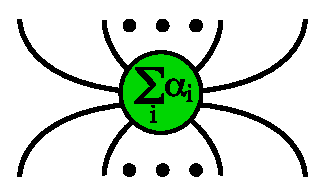
\includegraphics{images/gen-spider} = 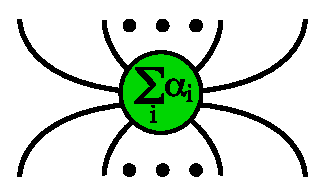
\includegraphics{images/gen-spider}
\label{fig:informal-spider-law}\caption{An informal equation on graphs
  that expresses the Spider Theorem. }
\end{figure}

Hence any connected subgraph involving nodes of only one colour,
wherever it occurs in a graph, may be collapsed to a single vertex
labelled by a single value $\alpha$, giving a ``spider''. Informally,
this can be depicted graphically as the equation in
Figure~\ref{fig:informal-spider-law}. Conversely, a spider may be
arbitrarily divided into subspiders, provided the total in- and
out-degree is preserved, along with and the sum of the $\alpha $s.
Further, one can derive, from the spider theorem, $n$-fold versions of
many of the other equations.

Spiders offer a very intuitive way to manipulate graphs, and are far
more compact and convenient in calculations than the graphs built up
naively from the generators.  However, formalising spiders requires
moving from finite graphs, where each vertex has bounded degree, and
which are subject to a finite number of rewrite rules, to a system
where nodes may have arbitrarily many edges, and there are infinitely
many concrete rewrite rules. The desire to retain these intuitive
reasoning methods motivates the extension from concrete graphs to
\emph{graph patterns}. These will comprise the main subject of this
paper.

\section{Graphs with Variable Nodes}

In the concrete representation, the following graphs represent
different computations:

\begin{center}
\inlinegraphic{2.5em}{compact1} \quad\quad
\inlinegraphic{2.5em}{compact3} \quad\quad
\inlinegraphic{2.5em}{compact5}
\end{center}

\noindent However, composition with semi-circles ($d$ and $e$ from
Definition~\ref{compactcat-def}), on the co-domain or domain, allows
an equation involving one of the above to easily lead to a derivation
corresponding to either of the other two. For instance, proving any of
the following allows a trivial derivation of the others:

\begin{center}
\inlinegraphic{2.5em}{compact1} $=$
\inlinegraphic{1.3em}{compact2} $\Leftrightarrow$
\inlinegraphic{2.5em}{compact3} $=$ \inlinegraphic{1.3em}{compact4}
$\Leftrightarrow$ \inlinegraphic{2.5em}{compact5} $=$
\inlinegraphic{2.5em}{comonoid-unit4}
\end{center}

\noindent This motivates a characterisation that has only one
representative for such a set of equations. More presicely, we
formalise a representation that abstracts over the boundary nodes
membership in the domain or co-domain. This gives rise to a
\emph{variable-node graphs}, in which boundary nodes have been
generalised to \emph{variable nodes}. The intuition of variable nodes
is that they can replaced by concrete nodes in some graph. This is a
process analgous to composition. We now define the semantics for
variable-node graphs and then go on and introduce a way to join them.

% relationship to composition on the underlying concrete graphs.


\subsection{Semantics by Matching as an Open Embedding}

To formalise the semantics of variable-node graphs, we define
matching, which captures the intuitive idea of a graph with variable
nodes occuring within another graph.

\begin{definition}
  \emph{Matching} is an open embedding
  (Definition~\ref{open-embedding-def}) which is strict for the
  non-variable nodes.
\end{definition}

A graph with variable nodes, $G$, can be given a formal semantics by
being interpretated as a set of concrete graphs, denoted by
$\vinterp{G}$. The interpretation is simply the set of concrete graphs
which the variable node graph matches. We refer to members of this set
as instances. Matching is also well-defined between two variable-node
graphs, in which case we denote that $G$ macthes $H$ by $G \leq_v H$.

\begin{theorem}
\label{match-interp-thm}
$G \leq_v H \Leftrightarrow \vinterp{G} \supseteq \vinterp{H}$. The
proof from left to right is a consequence of the trivial lemma that a
compositon of open embeddings is an open embedding. This makes the
embedding of $G$ into $H$ composed with $H$ into $\vinterp{H}$ an open
embedding of $G$ into $\vinterp{H}$. From right to left, we compose
the open embedding $\vinterp{G}$, restricted to it's subset
$\vinterp{H}$, with the inverse of $\vinterp{H}$ to get $G \leq_v H$.
\end{theorem}

\begin{theorem}
\label{reflexive-match-thm}
\emph{Matching is reflexive}: $G \leq_v G$ is a trivial instance of
the same theorem for open-embeddings, where the embedding is the
identity map.
\end{theorem}


% \begin{figure}[t]
% %  \scalebox{1.0}{\includegraphics{images/node-var-instance.eps}}
% *** Add figure *** 
% \label{node-variable-instances-fig}\caption{The concrete graphs $a$,
%   $b$, and $c$ are instances of $x$, a graph with variable nodes.}
% \end{figure}

% For example, in Figure~\ref{node-variable-instances-fig}, the graphs
% $a$, $b$ and $c$ are instances of the graph $x$. A graph with variable
% nodes, and without boundary nodes, is called a \emph{variable-node
%   graph}.

%% TYPES 
% Thus, unlike nodes in conrete a graph, variable nodes do not define an
% ordering on the edges that are incident. Instead, the edges that touch
% a variable node are simply a set. The type of a variable nodes is thus
% defined as a multiset rather than a tensor. Any tensor type can be
% lifted to a multiset type in the obvious manner, which we denote by
% the operation {\tt mset\_of\_tensor}. For example, {\tt
%   mset\_of\_tensor($a \tensor b \tensor a$) = $\{(a,2), (b,1)\}$}. We
% say that a tensor-type $T$ is an instance of a multiset type $M$,
% written $T \in M$, when $M \subseteq
% \mathtt{mset\_of\_tensor}(T)$. The intuition here is that when a
% variable node is instantiated to some other node, it's type will have
% at least the currently attached edges.

% An instance of a graph with variable nodes is the graph with every
% variable node replaced by a subgraph of the right type. When a graph
% has several varibale-nodes, the replacement subgraphs may be
% intersecting.

% \subsubsection{Completness and Adequacy.}

% Variable-node graphs are complete in the sense that for every concrete
% graph there is a variable node graph that can be instantiated to it:
% $\forall g.\,\exists G.\,g \in \vinterp{G}$. The witness for this
% proof is made by simply replacing all bounary nodes with variable
% nodes. 


%% not needed for this story...
%A variable node, $a$ is be said to an instance of another variable
%node $b$ when the multiset representing the type of $a$ is a superset
%of the multiset for the type of $b$. Thus, with regard to the
%underlying semantics, $a$ being a subtype of $b$ means that the set of
%instances of $a$ are a subset of the instances of $b$.



\subsection{Variable-node Plugging}

While concrete graphs can be composed sequentially as well as tensored
in an adjacent manner, variable-node graphs enjoy a single but
somewhat wilder joining operation which we call \emph{plugging}. 

\begin{definition}
  A \emph{plugging}, written $\pi_{p}(G,H)$, is a pair, $p$, of strict
  partial graph morphisms, $f_G : G \rightarrow H$ and $f_H : H
  \rightarrow G$ such that $f_G$ and $f_H$ \emph{agree}, following
  the definition given below, on node mappings and do not map concrete
  nodes.
\end{definition}

\begin{definition}
  Two mappings $f_G$ and $f_H$ \emph{agree} when $\forall v \in
  f_G(G).\, f_H(v) \in f^{-1}_G(v)$ and $\forall v \in f_H(H).\,
  f_G(v) \in f^{-1}_H(v)$. This states that if a set of nodes in one
  graph all map to a common node, $n$, in the other graph, then $n$
  maps back to one of the nodes that maps to it.
\end{definition}

We let $\pi(G,H)$ abbreviate $\exists p.\,\pi_p(G,H)$. We also
overload the notation $\pi_p(G,H)$ to denote the graph that results
from the plugging. This is defined to be the union of the nodes and
edges from $G$ and $H$ where the nodes and edges mapped by the pair of
plugging function are identified. Identification of nodes instantiates
variable nodes: when a variable node is mapped to a concrete one,
identification results in the concrete node.

While this is simply the intuitive way to combine graphs with variable
nodes, the definition takes some care. In particular, it is important
that plugging preserves incident edges of concrete nodes.
Figure~\ref{plugging-examples-fig} presents some examples to help the
reader get the intuition as well as understand some of the more
subtlte cases.

\begin{theorem}
  \emph{Plugging is symmetric}: $\forall p.\, \exists q.\, \pi_p(G,H)
  = \pi_q(H,G)$. Proof, given $p = (f_G,f_H)$ then $q = (f_H,f_G)$. As
  a corollary, we get $\pi(G,H) \Leftrightarrow \pi(H,G)$.
\end{theorem}

\begin{theorem}
  \emph{Plugging preserves matching}: $V \leq_v G \Rightarrow V \leq_v
  \pi_f(G,H)$. As corrolaries we get $V \leq_v H \Rightarrow V \leq_v
  \pi_f(G,H)$ from symmetry of plugging, $\vinterp{G} \cap \vinterp{H}
  \subseteq \bigcup_f \vinterp{\pi_f(G,H)}$ from the definition of
  interpretation, $G \leq_v \pi_f(G,H)$ from reflexivity of matching
  and consequently $H \leq_v \pi_f(G,H)$ by symmetry of plugging.
\end{theorem}

\section{!-Boxes}

A crucial feature of rules like the Spider Theorem is that an arbirary
number of repetitions of a subgraph need to be matched. To support
this we introduce an operation, !-boxing, on graph
representations. Given a graph representation, this introduces a new
notation by outlining (called !-boxing) a set of chosen
nodes. Intuitively, the resulting !-boxed graph can be thought of as
representing a set of graphs with an arbirary number of copies of the
!-boxed nodes, where every copy connects, in the same way, to the
nodes outside the !-box. The !-boxes can also be instantiated with
zero copies, which erases all edges to and from the !-box. See
Figure~\ref{spider-bang-rule} .

More formaly, a graph with !-boxes is a graph paired with a set
!-boxes. Each of these !-boxes is the set of nodes inside it and each
!-box must be disjoint from the others.\footnote{The disjointness
  condition avoids a slightly more complex, although also more
  expressive, semantics for overlaping node sets in the !-boxes. While
  such expressivity is interesting from a representational point of
  view, it is not needed to express the currently known rules of
  quantum computation.} 

For the purposes of this paper, the underlying graph representation of
!-boxed graphs is variable-node graphs. The set of variable-node
graphs for a graph $G$ with !-boxes, is denoted by $\binterp{G}$. We
now define the concept of !-box matching which we use to provide a
semantics for the !-boxed graphs.

\subsection{!-Matching.}

To formalise the intuitive notion that a !-box represents arbitrary
number of copies of the subgraph made from it's nodes, we introduce
\emph{!-box matching}. This is a binary relation on graphs, written
infix as $G \leq_! H$ when $G$ matches $H$. The set of !-box graphs
matched by a !-box graph is defined as the set closed by the following
operations on the !-boxes in a graph:

\begin{definition}
  \emph{copy}: copies a !-box, $b$ in a graph to produce a new graph
  with two copies of the !-boxed subgraph, $b$ is the old one and $b'$
  is the new one. The set of !-boxes in the copied graph now also
  contains the new !-box $b'$. Any edges between a node, $n$, inside
  the !-box $b$, and a node, $m$, outside it, get copied so that there
  is a new edge from $m$ to the new copy of $n$ in $b'$.
\end{definition}

\begin{definition}
  \emph{drop} simply removes the !-box, but leaves its contents in the
  graph.
\end{definition}

\begin{definition}
  \emph{kill} removes from the graph all nodes in the !-box as well as
  any incident edges.
\end{definition}

\begin{definition}
  \emph{merge} combines two !-boxes, $B_1$ and $B_2$ into a single
  larger !-box $B_1 \cup B_2$.
\end{definition}

\subsection{!-Box Semantics.} 

We give a formal semantics to a !-box graphs by defining the !-box
graph in terms of a set of graphs in the underlying representation. We
denote the interpretation of a !-box graph $G$ by $\binterp{G}$ and
say that members of $\binterp{G}$ are instances of $G$.

\begin{definition}
  \emph{Interpretation of !-box Graphs}: $\binterp{G}$ is the subset
  of graphs matched by the !-box graph that have no !-boxes.
\end{definition}

Observe that an instance of a !-box graph is defined by pairing each
!-box with the natural number that defines how many copies are made of
it. Thus the $\binterp{G}$ is isomorphic to the set of $k$-tuples of
natural numbers, where $k$ is the number of !-boxes.

\begin{theorem}
  \emph{!-Matching respects !-box semantics}: $G \leq_! H
  \Leftrightarrow \binterp{G} \supseteq \binterp{H}$. The proof is a
  simple consequence from the defintion of $\binterp{G}$ being a
  subset of the graphs that match $G$.
\end{theorem}


\section{Graph Patterns}
\label{sec:patterns}

The representation of Compact Closed Categories as Graphs, discussed
in~\S\ref{graph-repr-comp}, is too restrictive for reasoning about
quantum computation. In particular, pictures such the Spider Theorem, in
Figure~\ref{spider-law-fig} are frequently needed, but not
expressible. Such pictures are used to denote an infinite family of
concrete graphs that can be rewritten. In this section we combine the
{\em !-boxes} with {\em variable nodes} graph extensions to form a
representation that allows us to finitely express these infinite
families of concrete graphs. We call this extension \ref{graph
  patterns}. The Spider Law can now be represented by the equation in
Figure~\ref{graph-pattern-spider-law-fig}. We also extend the notion
of matching for graph pattens as well as present a corresponding
notion of plugging. This provides the foundations for the rewriting
machinery in~\S\ref{rewriting} which can then be used to reasoning
about quantum computation.

graph-pattern-spider-law-fig

\subsection{Matching}

The purpose of graph patterns is to formally express, in a declarative
manner, the intuitive idea of graph matching which commonly used in
quantum computation. To do this, we combine the two extensions to the
concrete graph representation, namely variable nodes and !-boxes, to
provides a matching relation between graph patterns and concrete
graphs as well as directly between graph patterns. The former relation
gives a semantics for our system and ensures soundness, while the
latter supports deirved equations and thus provides the theoretical
basis for our formulation of rewriting.

\subsubsection{Completeness.}

Graph patterns are complete in the sense that for every concrete graph
there is a pattern that matches it. This is a trivial consequence of
the completeness of variable-node extension to graphs, which is
unaffected by allowing !-boxes.


\subsubsection{Concrete Matches.}

The semantics for a graph pattern $G$ is a set of concrete graphs
denoted by $\minterp{G}$. We say that members of this set are
\emph{matched} by $G$. Formally, the concrete set of matches are
defined as:

$$\minterp{G} = \{\vinterp{G'}\;.\; G' \in \binterp{G}\}$$

\subsubsection{Graph Pattern Matches.}

The specification for one pattern matching another one is simply that
it is more general. Formally, a graph pattern, $G$, matches another
graph pattern, $H$, when $\minterp{G} \supseteq \minterp{H}$. This is
the specification for a matching algorithm which we implement of
in~\S\ref{sec:rewriting}. We can use the definition of open embedding
from variable-node graphs as an intermediate mechanism and show that a
suitable definition of graph pattern matching is simply the !-Box
matching followed by variable-node matching:

\begin{definition}
  $G \leq H \Leftrightarrow \forall H' \in \binterp{H}.\,\exists G' \in \binterp{G}.\, G' \leq_v H'$
\end{definition}

Because viable-node matching preserves the semantics, it is trivial to
prove that this definition meets the specification. This gives us
matching between pattern-nodes.

\subsubsection{Graph Pattern Equality.}

Equality of graph patterns can simply be defined as mutual matching: 

\begin{definition}
  $G = H \Leftrightarrow G \leq H \land H \leq G$
\end{definition}


\subsection{Plugging}

We then extend the plugging
operation on variable-node graphs to graphs with !-boxes.


By defining graph patterns as a conservative extension of concrete
graphs we get the relative soundness for them.



\section{Reasoning with Graph Patterns}
\label{sec:rewriting}

In this section we describe how the garph pattern formalism can
provide a \emph{meta-level} framework for reasoning about models of
compact closed categories. Following the terminology of logical
frameworks such as Isabelle~\cite{isabelle}, we call the specification
provided by the underlying model an \emph{object-level} graph
formalism. In particular, an object-level formalisation defines a set
of rules which are treated as the axioms for the system. It also
defines the data at the nodes and edges as well as corresponding
data-matching behaviour. For it's part, the meta-level provides
machinery to manipulate graphs and derive new rules. In this section
we describe the meta-level framework and prove its adequacy for
rewriting.

\subsection{Equational Rules}

Axioms defined by an object-level model, as well as derived rules in
our framework, are pairs of pattern graph. The pair represents the
left and right hand sides of an equation. Rules are declarative in
that they denote set of concrete equational rules. 

Substituon with a rule involves replacing a subgraph that matches the
left hand side with the right hand side. To do this there has to be a
isomorphism between variable nodes in the left and right hand
subgraphs. More concretely, there must be a unique naming of the
variable nodes in the left hand side such that each name occurs in a
unique variable node on the right hand side. Given a matching on the
left hand side, the target subgraph is replaced with the right hand
side while keeping the same instantiations for the isomorphic variable
nodes. 

Rules also contain a partial 1-1 mapping between !-boxes on the left
and right hand sides. The intuition for this mapping is that the
unfolding used when matching, for a !-box on the left, is applied to
the mapped !-box on the right before replacement. 

Notationally, and implementationally, we annotate !-boxes and variable
nodes in a graphs with unique names. For example,
Figure~\ref{spider-law2-fig} illustrates the Spider Law as a rule in
the general framework. The partial 1-1 mapping for !-boxes is
represented by !-boxes having the same name on the left and right of a
rule. Similarly, the isomorphism between variable nodes is captured by
the set of variable node names on the left and right hand side being
equal. There is an additional restriction that comes from the
interplay between !-boxes and variable nodes. When a variable node
appears within a !-box on one side of a rule it must appear under
mapped !-box on the other side. This enforces that rules cannot change
the type of a graph pattern.

\subsection{Adequacy}

This
provides rewriting for pattern graphs.

A an equation on a graph pattern is 

\emph{Adequacy} says that if one by doing so within an
equation, we are not


\subsection{Meta-Level Logic and Derived Rules}

The meta-logical rules of the framework are quite simple as they only
involve dealing with object-level equations:

\begin{center}
\prooftree
A = B \in \Gamma
\justifies
\Gamma \vdash A = B
\using\mbox{trivial}
\endprooftree
\quad\quad
\prooftree
\justifies
\Gamma \vdash A = A
\using\mbox{reflexivity}
\endprooftree
\end{center}

\begin{center}
\prooftree
\Gamma \vdash A = B
\justifies
\Gamma \vdash B = A
\using\mbox{symmetry}
\endprooftree
\quad\quad
\prooftree
\Gamma \vdash A = B
\Gamma \vdash C = D
\justifies
\Gamma \vdash (C = D[A/B])
\using\mbox{substitution}
\endprooftree
\end{center}

\noindent where $\Gamma$ is the set of object-level axioms. For the
reflexivity rule, $A$ must be a well-formed pattern graph. 

This system allows derived rules which allow a combination of steps to
be abbreviated by representing them as a single new rule. 

\subsection{Soundness and Completeness} 

The soundness of a system that uses our meta-level rests on two
arguments: 

\begin{itemize}
\item Representation of the underying model as a compact closed
  category with a defined set of equations.

\item The soundness and adequacy of the axioms when expressed within
  the compact closed category. Adquency ensures that the encoding as a
  graph pattern represents only the intended concrete rules. The
  soundness of the rules is obviously needed and requires proving the
  rule in terms of the underlying semantics.
\end{itemize}

The proof of adequancy ...

The completeness of the resulting system, with respect to the intended
underlying semantics, depends on the completeness of the set of given
rules.

\subsection{Derived Rules}


\subsection{Simplification}


\subsection{Adequacy}





% An object-level graph system is sound if their is some pair of graphs
% which can not be derived as an equation.

% To ensure soundness, it is sufficient to show that the object-level
% model is a compact-closed category and that the basic equational rules
% of the object-level can be proved in the underlying model.

% The axioms should be proved of the particular model of concrete graphs
% being considered.

% \subsubsection{Completeness.} A formalism for graphs can be shown to
% be complete with respect to the underlying semantics if the equational
% rules have been shown to be complete. 

% \subsection{Implications}


\section{A Case Study in Quantum Computation}

The model of qantum computation in which we are interested is finite
dimensional hilbert spaces. 

\subsection{Node Expressions}
\label{ssec:node-expressions}


Completeness is a challenging and still open problem for graph based
models of quantum computation. However, even without completeness
interesting quantum computations can be expressed.


\section{Related Work}
\label{sec:relatedwork}

Initially one might be tempted to think that the usual notion of
subgraph might surfice for expressing matching, however it allows
additional edges on nodes where, because of the tensorial semantics of
our graphs, we do not. Our work provides a restriction of the usual
subgraph definition that is sound for Compact Closed Categories.

Link Graphs and their extention to BiGraphs also encapsualte a very
different kind of semantics where they allow edges to go to multiple
nodes. An interesting area of further work would be to consider our
graph patterns for these, and other, graph based formalisms.

Graph Grammars...

Other graph rewriting... 

Matrix Based Graph Tansformation...

Other Graph Transformation...

Interaction nets and interaction combinators (Lafont and others)

\section{Conclusions}
\label{sec:conclusions}

Ideas for further work
\begin{itemize}
\item simplification ordering
\item confluence arguments for graphs
\item formalise algorithms in a thm prover
\item richer graph structures - quantification over edges
\item richer expression language in vertices
\item completeness of rewrite rules with respect to wpHilb
\end{itemize}

\bibliographystyle{plain}
\bibliography{all,bibfile}

\end{document}



